\documentclass[t]{beamer}
\usetheme[english]{KIT}

\usepackage{amssymb} %% For \backprime
\usepackage{multicol}

%\usepackage{mathpartir}
\usepackage{graphicx}

\usepackage{tikz}
\usetikzlibrary{arrows.meta,positioning,calc}

\usepackage[T1]{fontenc}
\usepackage{babel}
\usepackage{booktabs}
\usepackage[normalem]{ulem}
\usepackage{fontspec}
\setmonofont[Scale=MatchLowercase]{Iosevka}
%\newfontfamily\lc[Scale=MatchLowercase]{Iosevka SS09}

\usepackage{minted}
\definecolor{codebg}{rgb}{0.95,0.95,0.95}
\setminted{bgcolor=codebg,breaklines}
\usemintedstyle{tango}
\newmintinline[lean]{lean}{bgcolor=white}
\newminted{lean}{fontsize=\footnotesize}

\usepackage{newunicodechar}
\newfontfamily{\freeserif}{DejaVu Sans}
\newunicodechar{ℕ}{\freeserif{ℕ}}
\newunicodechar{ℝ}{\freeserif{ℝ}}
\newunicodechar{ₐ}{\freeserif{ₐ}}
%\newunicodechar{₁}{\freeserif{₁}}
%\newunicodechar{∈}{\freeserif{∈}}
\newunicodechar{𝓞}{\ensuremath{\mathcal{O}}}
\newunicodechar{∉}{\freeserif{∉}}
%\newunicodechar{Π}{\freeserif{Π}}
%\newunicodechar{→}{\freeserif{→}}
\newunicodechar{⦃}{\freeserif{⦃}}
\newunicodechar{⦄}{\freeserif{⦄}}
%\newunicodechar{∧}{\freeserif{∧}}
%\newunicodechar{∨}{\freeserif{∨}}
%\newunicodechar{⊢}{\freeserif{⊢}}
\newunicodechar{⊑}{\freeserif{⊑}}
\newunicodechar{ₚ}{\freeserif{ₚ}}
\newunicodechar{∘}{\freeserif{∘}}
\newunicodechar{ₗ}{\freeserif{ₗ}}
\newunicodechar{∪}{\freeserif{∪}}
\newunicodechar{⋃}{\freeserif{⋃}}
\newunicodechar{𝓸}{\ensuremath{o}}
\newunicodechar{⊆}{\freeserif{⊆}}
\newunicodechar{≼}{\freeserif{≼}}
\newunicodechar{≃}{\freeserif{≃}}

% https://github.com/gpoore/minted/issues/220
\AtBeginEnvironment{snugshade*}{\vspace{-0.4\FrameSep}}
%\AfterEndEnvironment{snugshade*}{\vspace{-0.8\FrameSep}}

% https://tex.stackexchange.com/questions/343494/minted-red-box-around-greek-characters
\makeatletter
\AtBeginEnvironment{minted}{\dontdofcolorbox}
\def\dontdofcolorbox{\renewcommand\fcolorbox[4][]{##4}}
\makeatother

\title{Embedding Languages into Lean 4}

\author[Ullrich]{Sebastian Ullrich}
\subtitle{\insertauthor}
\institute[IPD Snelting]{Programming paradigms group - IPD Snelting}
\date{2020/02/02}
\makeatletter
\sbox{\KIT@titimg}{
  \hspace{0.08\titleimagewd}
    \raisebox{0.1\titleimageht}{
      \includegraphics[height=0.8\titleimageht]{logo}
    }
}

\newcommand{\kit}[1]{\textcolor{KITgreen}{#1}}

\begin{document}
\begin{frame}
  \maketitle
\end{frame}

\begin{frame}{Lean is ...}
  yet another dependently-typed theorem prover
\end{frame}

\begin{frame}{Lean is ...}
  \begin{itemize}
  \item opinionated
    \begin{itemize}
    \item implements a single logic: CIC with proof irrelevance and quotient types
      \begin{itemize}
      \item good for automation, great for classical mathematics
      \item not good for metatheoretic properties \pause
      \item ``We're not in the type theory research business''
      \end{itemize}
      \pause
    \item typeclasses as the main abstraction interface
    \end{itemize}
    \pause\vfill
  \item ``modern''/un-arcane
    \begin{itemize}
    \item unobtrusive syntax heavily reliant on Unicode
    \item good integration into VS Code
    \item simple tooling that ``mostly just works'': leanpkg, elan
    \end{itemize}
    \pause\vfill
  \item welcoming
    \begin{itemize}
    \item excellent introductory text: Theorem Proving in Lean
      \begin{itemize}
      \item comes with passable online editor
      \end{itemize}
    \item \emph{huge} friendly crowd on the Zulip chat
      \begin{itemize}
      \item real-time chat with beginners-only section is crucial
      \end{itemize}
    \end{itemize}
  \end{itemize}
\end{frame}

\begin{frame}{A brief history of Lean}
  \begin{itemize}
  \item Lean 0.1 (2014)
  \item Lean 2 (2015)
    \begin{itemize}
    \item first official release
    \item fixed tactic language
    \end{itemize}
  \item Lean 3 (2017)
    \begin{itemize}
    \item make Lean a \kit{meta-programming} language: build tactics in Lean
    \item backed by a bytecode interpreter
    \end{itemize}
  \item Lean 4 (202X)
    \begin{itemize}
    \item make Lean a \kit{general-purpose} language: native back end, FFI, ...
    \item reimplement Lean in Lean
    \end{itemize}
  \end{itemize}
\end{frame}

%\begin{frame}
%  \vfill
%  \includegraphics[width=\textwidth]{when}
%  \vfill
%\end{frame}

\begin{frame}{Towards a fully extensible frontend}
  Goal: \emph{democratize} frontend by removing the barrier between built-in and user-defined notions
  \begin{itemize}
    \pause
  \item extensible syntax from simple mixfix notations to character-level parsing
    \pause
  \item extensible semantics from simple syntax sugars to type-aware elaboration
    \pause
  \item extensible tooling with access to frontend metadata
    \begin{itemize}
    \item concrete syntax tree
    \item elaboration annotations (TBD)
    \end{itemize}
  \end{itemize}
  \pause
  \bigskip
  Non-goal: extensible type theory
\end{frame}

\begin{frame}[fragile]{Frontend: overview}
  \begin{center}
    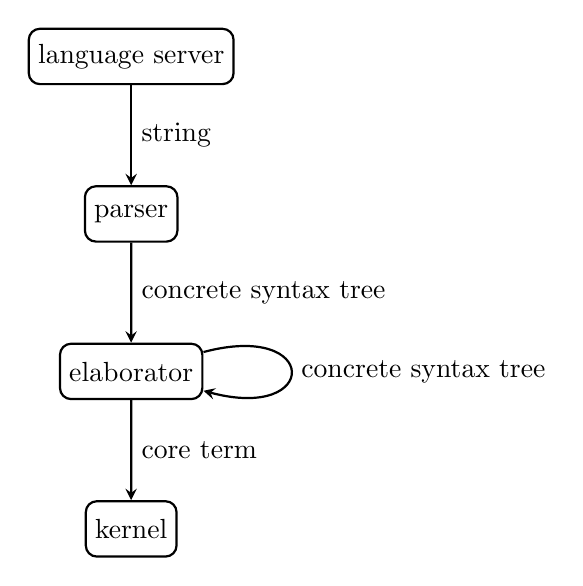
\begin{tikzpicture}[>=stealth, thick, nodes={rounded corners, minimum height=2em}, level distance=20mm]
      \node[draw] {language server}
      child[->] {
        node[draw] (parser) {parser}
        child {
          node[draw]  (elab) {elaborator}
          child[->] {
            node[draw] {kernel}
            edge from parent node[right] {core term}
          }
          edge from parent node[right] {concrete syntax tree}
        }
        edge from parent node[right] {string}
      };
      \draw[->,loop right] (elab) to node {concrete syntax tree} (elab);
    \end{tikzpicture}
  \end{center} 
\end{frame}

\begin{frame}[fragile]{Concrete syntax tree}
  provide
  \begin{itemize}
  \item precise source locations
  \item whitespace and comments
  \item erroneous input
  \end{itemize}
  for
  \begin{itemize}
  \item code editors
  \item documentation generators
  \item code formatters
  \item refactoring tools
  \item better LaTeX highlighting...
  \end{itemize}
\end{frame}

\begin{frame}[fragile,fragile]{Extensible concrete syntax tree}
\begin{leancode}
inductive Syntax
| atom   (info : Option SourceInfo) (val : String)
| ident  (info : Option SourceInfo) (rawVal : Substring) (val : Name) (preresolved : List (Name × List String))
| node   (kind : SyntaxNodeKind) (args : Array Syntax)
| missing

structure SourceInfo :=
(leading  : Substring)
(pos      : String.Pos)
(trailing : Substring)

abbrev SyntaxNodeKind := Name
\end{leancode}

\begin{leancode}
a -> b
\end{leancode}

\begin{leancode}
(Term.arrow `a "->" `b)
\end{leancode}
\end{frame}

\begin{frame}{Parser}
  \begin{itemize}
  \item Lean 3: basic lexer, LL(1) recursive descent parser
  \item Isabelle: basic lexer, Earley parser for arbitrary context-free grammars, delimited terms
    \pause
  \item Lean 4: arbitrary, character-based parser; combinators including Pratt
    parser and longest-prefix matching
    \pause
    \begin{itemize}
    \item problem: monadic parser combinators allocate like crazy, lexing should
      be cached
    \end{itemize}
  \end{itemize}
\end{frame}

\begin{frame}[fragile]{Parser state}
\begin{leancode}
def ParserFn := ParserContext → ParserState → ParserState

structure ParserContext :=
(input    : String)
(fileName : String)
(env      : Environment)
(tokens   : TokenTable)

structure ParserState :=
(pos      : String.Pos)
(cache    : ParserCache)
(errorMsg : Option Error)
(stxStack : Array Syntax)
\end{leancode}
\end{frame}

\begin{frame}[fragile,fragile,fragile]{Parser: syntax stack}
\begin{leancode}
def nodeFn (k : SyntaxNodeKind) (p : ParserFn) : ParserFn :=
fun c s =>
  let iniSz := s.stxStack.size;
  let s     := p c s;
  let stack := s.stxStack;
  let newNode := Syntax.node k (stack.extract iniSz stack.size);
  let stack   := stack.shrink iniSz;
  let stack   := stack.push newNode;
  { s with stxStack := stack }
\end{leancode}
  
\begin{leancode}
nodeFn `Term.arrow (identFn >> symbolFn "->" >> identFn)
\end{leancode}

\begin{leancode}
   [..., `a, "->", `b]
~> [..., (Term.arrow `a "->" `b)]
\end{leancode}
\end{frame}

\begin{frame}[fragile]{Parser: token caching}
  cache last ``token'' read
\begin{leancode}
def tokenFn : ParserFn :=
fun c s =>
  let i := s.pos;
  let tkc := s.cache.tokenCache;
  if tkc.startPos == i then
    let s := s.pushSyntax tkc.token;
    s.setPos tkc.stopPos
  else
    let s := tokenFnAux c s;
    updateCache i s
\end{leancode}
\end{frame}

\begin{frame}[fragile]{Parser: token caching}
\begin{leancode}
def identFn : ParserFn :=
fun c s =>
  let iniPos := s.pos;
  let s      := tokenFn c s;
  if s.hasError || !s.stxStack.back.isIdent then s.mkErrorAt "identifier" iniPos else s
\end{leancode}
  \vspace{-5mm}
  \pause
\begin{leancode}
structure Parser :=
(fn   : ParserFn)
(info : ParserInfo)

structure ParserInfo :=
(collectTokens : List TokenConfig → List TokenConfig   := id)
(firstTokens   : FirstTokens                           := FirstTokens.unknown)

structure TokenConfig :=
(val     : String)
(lbp     : Option Nat)
\end{leancode}
\end{frame}

\begin{frame}[fragile]{Pratt parser}
  token-indexed precedence parsing with longest-match semantics
\begin{leancode}
def prattParser (tables : PrattParsingTables) (rbp : Nat := 0) : ParserFn

structure PrattParsingTables :=
(leadingTable    : TokenMap Parser)
(leadingParsers  : List Parser)
(trailingTable   : TokenMap Parser)
(trailingParsers : List Parser)

def leadingParser (tables : PrattParsingTables) : ParserFn :=
fun c s =>
  let (s, ps) := indexed tables.leadingTable c s;
  let ps      := tables.leadingParsers ++ ps;
  longestMatchFn ps c s
\end{leancode}
\end{frame}

\begin{frame}[fragile]{Actual stdlib parsing}
  \emph{Syntactic categories} are Pratt parsers extensible via attributes
\begin{leancode}
@[init] def regTermCat : IO Unit :=
registerSyntaxCategory `term

def term (rbp : Nat := 0) : Parser :=
categoryParser `term rbp

@[termParser] def anonymousCtor := node `Term.anonymousCtor (
  symbol "⟨" appPrec >> sepBy term ", " >> "⟩")

def optIdent : Parser := optional (try (ident >> " : "))
@[termParser] def «if»  := node `Term.if (
  "if " >> optIdent >> term >> " then " >> term >> " else " >> term)
\end{leancode}
\end{frame}

\begin{frame}[fragile]{Actual stdlib parsing}
  \emph{Syntactic categories} are Pratt parsers extensible via attributes
\begin{leancode}
declare_syntax_cat term

syntax "⟨" (sepBy term ", ") "⟩" : term

syntax optIdent := (try (ident " : "))?
syntax "if " optIdent term " then " term " else " term : term
\end{leancode}
\end{frame}

\begin{frame}[fragile,fragile,fragile]{Macros}
\begin{leancode}
syntax "if " optIdent term " then " term " else " term : term
\end{leancode}
Apply meaning to syntax via recursive syntactic substitutions (or \emph{macros}):
\begin{leancode}
macro_rules
| `(if $h : $cond then $t else $e) => `(dite $cond (fun $h => $t) (fun $h => $e))
| `(if $cond then $t else $e)      => `(if h : $cond then $t else $e)
\end{leancode}
\begin{onlyenv}<2>
\begin{leancode}
if True then h else True.intro
\end{leancode}
\end{onlyenv}
\begin{onlyenv}<3-4>
\begin{leancode}
if True then h else True.intro  -- unknown identifier 'h'
\end{leancode}
\end{onlyenv}
\begin{onlyenv}<4>
  Lean 4 macros are \emph{hygienic} $\Rightarrow$ \lean{dite} resolved in the declaration context, references in \lean{t} in the caller context, ...
\end{onlyenv}
\end{frame}

\begin{frame}[fragile,fragile]{Macros!}
\begin{leancode}
syntax [if] "if " optIdent term " then " term " else " term : term
\end{leancode}

\begin{leancode}
@[macro «if»] def expandIf (stx : Syntax) : MacroM Syntax :=
match_syntax stx with
| `(if $h : $cond then $t else $e) => `(dite $cond (fun $h => $t) (fun $h => $e))
| `(if $cond then $t else $e)      => `(if h : $cond then $t else $e)
| _                                => throwUnsupportedSyntax
\end{leancode}
  \only<1>{Macros can be arbitrary \emph{syntax transformers}}
  \pause
  Hygiene is tied to syntax quotations, which are \emph{monadic values}
\begin{leancode}
class MonadQuotation (m : Type → Type) :=
(getCurrMacroScope : m MacroScope)
\end{leancode}
  \lean{`(...) : m Syntax} given \lean{[MonadQuotation m]}
\end{frame}

\begin{frame}[fragile]{Macros!!}
\begin{leancode}
syntax [if] "if " optIdent term " then " term " else " term : term
\end{leancode}

\begin{leancode}
@[termElab «if»] def elabIf : TermElab :=
adaptMacro $ fun stx => match_syntax stx with
| `(if $h : $cond then $t else $e) => `(dite $cond (fun $h => $t) (fun $h => $e))
| `(if $cond then $t else $e)      => `(ite $cond $t $e)
| _                                => throwUnsupportedSyntax

def adaptMacro (exp : Syntax → MacroM Syntax) : TermElab :=
fun stx expectedType? => do
  stx' ← exp stx;
  elabTerm stx' expectedType?

def elabTerm (stx : Syntax) (expectedType? : Option Expr) : TermElabM Expr
\end{leancode}
  Lean 4 macros are actually just ``tail-recursive elaborators''
\end{frame}

\begin{frame}[fragile]{Macros!!!}
\begin{leancode}
syntax [anonCtor] "⟨" (sepBy term ", ") "⟩" : term
\end{leancode}

\begin{leancode}
@[termElab anonCtor] def elabAnonCtor : TermElab :=
fun stx expectedType? => match_syntax stx with
| `(⟨$args*⟩) => do
  tryPostponeIfNoneOrMVar expectedType?;
  match expectedType? with
  | some expectedType => do
    match Expr.getAppFn expectedType with
    | Expr.const constName _ _ => do
      ctors ← getCtors constName;
      match ctors with
      | [ctor] => do
        stx ← `($(mkCTermId ctor) $(getSepElems args)*);
        elabTerm stx expectedType?
...  -- error handling
\end{leancode}
\end{frame}

\begin{frame}{Macros?}
  \vfill
  \includegraphics[width=\textwidth]{macro}
  \vfill
\end{frame}

\begin{frame}
  \vfill
  \begin{center}
    \Huge\textbf{Demo}
  \end{center}
  \vfill
\end{frame}

\begin{frame}{Conclusion}
  \begin{itemize}
  \item arbitrarily extend the Lean language using a tower of abstraction levels
    \bigskip
  \item extend Lean with other languages... with some preliminary caveats
    \begin{itemize}
    \item token handling should be refined and made customizable
    \end{itemize}
  \end{itemize}
\end{frame}

% \tikzset{
%  invisible/.style={opacity=0},
%  visible on/.style={alt={#1{}{invisible}}},
%  alt/.code args={<#1>#2#3}{%
%    \alt<#1>{\pgfkeysalso{#2}}{\pgfkeysalso{#3}} % \pgfkeysalso doesn't change the path
%  },
%}
%
%\newcommand<>{\lol}[3]{
%  \fill[#1!20] (path picture bounding box.north west)rectangle (path picture bounding box.south east);
%  \alt#4{\fill[#1!50] (path picture bounding box.north west)rectangle ($(path picture bounding box.south west)!#3!(path picture bounding box.south east)$);}
%  {\fill[#1!50] (path picture bounding box.north west)rectangle ($(path picture bounding box.south west)!#2!(path picture bounding box.south east)$);}
%  }
%
%\begin{frame}[fragile]
%  \only<1>{\frametitle{Lean 4 progress: Jan 2019}}
%  \only<2>{\frametitle{Lean 4 progress: Jun 2019}}
%  \only<3>{\frametitle{Lean 4 progress: Dec 2019}}
%  \only<4>{\frametitle{Lean 4 progress: Jan 2020}}
%  \begin{center}
%    \begin{tikzpicture}[>=stealth, thick, nodes={rounded corners, minimum height=2em}, level distance=12mm]
%      \node[draw,fill=red!50][path picture={\lol<1>{red}{0}{0}}] (editor) {editor}
%        child[<->] {
%          node[draw,fill=blue!50][path picture={\lol<1>{green}{0}{0}}] {language server}
%          child[->] {
%            node[draw,fill=blue!50][path picture={\lol<2->{green}{0.8}{1}}] (parser) {parser}
%            child {
%              node[draw,fill=blue!50] [path picture={\lol<4->{green}{0.1}{0.5}}] (elab) {elaborator}
%              child[->] {
%                node[draw,fill=blue!50][path picture={\lol<1>{blue}{1}{1}}] {kernel}
%              }
%              child[->] {
%                node[draw,fill=blue!50][path picture={
%                  \lol<1>{blue}{0.8}{0.8}
%                  \only<2->{
%                    \fill[blue!50,sharp corners] (path picture bounding box.north west)rectangle ($(path picture bounding box.north east)!0.7!(path picture bounding box.south east)$);
%                    \fill[green!50,sharp corners] ($(path picture bounding box.north west)!0.7!(path picture bounding box.south west)$)rectangle (path picture bounding box.south east);
%                  }
%}] (comp) {compiler}
%              }
%              edge from parent[draw=none]
%            }
%          }
%        };
%        \node[draw,right=of elab][path picture={\lol<4->{green}{0}{0.1}}] (tac) {tactic framework};
%      \node[draw,fill=green!20,left=of elab][path picture={
%        \only<3->{
%        \fill[blue!50,sharp corners] (path picture bounding box.north west)rectangle ($(path picture bounding box.north east)!0.2!(path picture bounding box.south east)$);
%        \fill[green!50,sharp corners] ($(path picture bounding box.north west)!0.2!(path picture bounding box.south west)$)rectangle (path picture bounding box.south east);
%        }
%}] (mod) {module system};
%      \uncover<3->{
%        \node[draw,above=3mm of mod][path picture={\lol<1>{green}{1}{1}}] {meta monad};
%        \node[draw,below=3mm of mod][path picture={\lol<1>{green}{1}{1}}] {typeclass resolution};
%      }
%      \alt<1>{
%        \node[draw,right=of parser][path picture={\lol<2->{green}{0.5}{1}}] (mac) {macro expander};
%        \draw[->] (parser) to (mac);
%        \draw[->] (mac) to (elab);
%      }{
%        \node[draw,right=of parser][path picture={\lol<2->{green}{0.7}{1}}] (mac) {macro hygiene};
%        \draw[->] (parser) to (elab);
%        \draw[-] (mac) to (elab);
%      }
%      \node[draw,below=3mm of comp][path picture={\lol<1>{blue}{0}{0}}] (ffi) {FFI};
%      \draw[-] (comp) to (ffi);
%      \only<3->{
%        \node[draw,right=of ffi][path picture={\lol<1>{blue}{1}{1}}] (interp) {interpreter};
%        \draw[-] (comp) to (interp);
%      }
%      \draw[->] (comp) to (tac);
%      \draw[->] (tac) to (elab);
%      \node[draw,left=35mm of editor,yshift=5mm,minimum height=5mm,minimum width=5mm][path picture={
%        \fill[blue!20] (path picture bounding box.north west)rectangle (path picture bounding box.south east);
%        \fill[blue!50] (path picture bounding box.north west)rectangle ($(path picture bounding box.south west)!0.5!(path picture bounding box.south east)$);
%        }] (cpp) {};
%        \node[right=1mm of cpp] {C++};
%      \node[draw,below=1mm of cpp,minimum height=5mm,minimum width=5mm][path picture={
%        \fill[green!20] (path picture bounding box.north west)rectangle (path picture bounding box.south east);
%        \fill[green!50] (path picture bounding box.north west)rectangle ($(path picture bounding box.south west)!0.5!(path picture bounding box.south east)$);
%        }] (lean) {};
%        \node[right=1mm of lean] {Lean};
%      \node[draw,below=1mm of lean,minimum height=5mm,minimum width=5mm][path picture={
%        \fill[red!20] (path picture bounding box.north west)rectangle (path picture bounding box.south east);
%        \fill[red!50] (path picture bounding box.north west)rectangle ($(path picture bounding box.south west)!0.5!(path picture bounding box.south east)$);
%        }] (other) {};
%        \node[right=1mm of other] {other};
%    \end{tikzpicture}
%  \end{center} 
%\end{frame}
%
%\begin{frame}[fragile]{Cosmetics}
%  Minor syntax changes to make Lean a more consistent and pleasant language
%  \bigskip
%
%  \begin{itemize}
%  \item<+-> naming convention: \texttt{TypeName},  \texttt{ModuleName}, \texttt{termName}
%    \begin{itemize}
%    \item<+-> lemma convention \verb!termName_property_of_assumption!?
%    \end{itemize}
%  \item<+-> consistent pattern syntax
%    \vspace{-4mm}
%    \begin{columns}
%      \column{0.4\textwidth}
%      \begin{leancode}
%def hiThere : ...
%| pat1, ... => ...
%| ...
%\end{leancode}
%      \column{0.4\textwidth}
%\begin{leancode}
%match ... with
%| pat1, ... => ...
%| ...
%\end{leancode}
%    \end{columns}
%  \item<+-> etc...
%\begin{leancode}
%fun x =>
%  let y := 1;
%  do a; b
%\end{leancode}
%  \end{itemize}
%\end{frame}
%
%\begin{frame}{Compiler}
%  Ullrich and de Moura. \emph{Counting Immutable Beans: Reference Counting Optimized for Purely Functional Programming}. IFL'19.
%  
%  \includegraphics[width=\textwidth]{bench}
%\end{frame}
%
%\begin{frame}{New typeclass resolution}
%  Performance issues with the old implementation:
%  \begin{itemize}
%  \item \emph{diamonds} can lead to exponential runtime
%  \item cycles can lead to nontermination
%  \end{itemize}
%  \pause
%  \bigskip
%
%  Typeclass resolution follows a ``Prolog-like search''
%  \pause
%  
%  $\Rightarrow$ adapt known Prolog optimization, \emph{tabled resolution}, to Lean!
%  
%  \begin{center}
%    \includegraphics[height=0.5\textheight]{resolv}
%  \end{center}
%
%  Guarantees termination if size of typeclass problems is bounded
%\end{frame}
%
%%\begin{frame}[fragile]{New typeclass resolution: benefits for users}
%%  \begin{itemize}
%%  \item guarantees termination if size of typeclass problems is bounded
%%  \item no need for transitive helper classes such as \texttt{HasCoeT}
%%  \item \texttt{HasCoe a b} and \texttt{HasCoe b a} are simultaneously permissible
%%  \end{itemize}
%%  \bigskip
%%
%%\begin{leancode}
%%instance coeTrans {α β γ : Type} [HasCoe β γ] [HasCoe α β] : HasCoe α γ
%%instance coeBoolToProp : HasCoe Bool Prop
%%instance coeDecidableToBool (p : Prop) [Decidable p] : HasCoe
%%instance coeSubtype {α : Type} {p : α → Prop} : HasCoe {x // p x} α
%%\end{leancode}
%%\end{frame}
%
%\begin{frame}[fragile]{State of the ⋃}
%  \begin{onlyenv}<+-+(1)>
%\begin{leancode}
%notation "⋃ " binders ", " r:(scoped f, Union f) := r
%\end{leancode}
%    \vspace{-5mm}
%    \begin{onlyenv}<+>
%\begin{leancode}
%expected ':='
%\end{leancode}
%    \end{onlyenv}
%  \end{onlyenv}
%  \begin{onlyenv}<+>
%\begin{leancode}
%notation "⋃ " b ", " r := Union (fun b => r)
%
%
%#check ⋃ x,              x = x
%#check ⋃ (x : Set Unit), x = x
%#check ⋃ x ∈ univ,       x = x   -- error
%\end{leancode}
%  \end{onlyenv}
%  \begin{onlyenv}<+>
%\begin{leancode}
%notation "⋃ " b ", " r := Union {b | r}
%
%
%#check ⋃ x,              x = x
%#check ⋃ (x : Set Unit), x = x
%#check ⋃ x ∈ univ,       x = x   -- works!
%\end{leancode}
%  \end{onlyenv}
%  \begin{onlyenv}<+-+(1)>
%\begin{leancode}
%syntax "⋃ " term ", " term : term
%macro `(⋃ $b, $r) => `(Union {$b | $r})
%
%#check ⋃ x,              x = x
%#check ⋃ (x : Set Unit), x = x
%#check ⋃ x ∈ univ,       x = x   -- works!
%\end{leancode}
%    \vspace{-5mm}
%    \begin{onlyenv}<+>
%\begin{leancode*}{stripnl=false}
%
%
%
%syntax "{" term " | " term "}" : term
%macro
%| `({$x ∈ $s | $p}) => `(setOf (fun $x => $x ∈ $s ∧ $p))
%| `({$x ≤ $e | $p}) => `(setOf (fun $x => $x ≤ $e ∧ $p))
%
%| `({$b      | $r}) => `(setOf (fun $b => $r))
%\end{leancode*}
%    \end{onlyenv}
%  \end{onlyenv}
%  \begin{onlyenv}<+>
%\begin{leancode}
%syntax "⋃ " setIdx ", " term : term
%macro `(⋃ $b, $r) => `(Union {$b | $r})
%
%#check ⋃ x,              x = x
%#check ⋃ x : Set Unit,   x = x  -- works!
%#check ⋃ x ∈ univ,       x = x
%\end{leancode}
%    \vspace{-5mm}
%\begin{leancode*}{stripnl=false}
%
%
%
%syntax "{" term " | " term "}" : term
%macro
%| `({$x ∈ $s | $p}) => `(setOf (fun $x => $x ∈ $s ∧ $p))
%| `({$x ≤ $e | $p}) => `(setOf (fun $x => $x ≤ $e ∧ $p))
%
%| `({$b      | $r}) => `(setOf (fun $b => $r))
%\end{leancode*}
%  \end{onlyenv}
%  \begin{onlyenv}<+>
%\begin{leancode}
%syntax "⋃ " setIdx ", " term : term
%macro `(⋃ $b, $r) => `(Union {$b | $r})
%
%#check ⋃ x,              x = x
%#check ⋃ x : Set Unit,   x = x  -- works!
%#check ⋃ x ∈ univ,       x = x
%\end{leancode}
%    \vspace{-5mm}
%\begin{leancode}
%declare_syntax_cat setIdx
%syntax term                      : setIdx
%syntax ident " : " term          : setIdx
%syntax "{" setIdx " | " term "}" : term
%macro
%| `({$x ∈ $s | $p}) => `(setOf (fun $x => $x ∈ $s ∧ $p))
%| `({$x ≤ $e | $p}) => `(setOf (fun $x => $x ≤ $e ∧ $p))
%| `({$x : $t | $r}) => `(setOf (fun ($x : $t) => $r))
%| `({$b      | $r}) => `(setOf (fun $b => $r))
%\end{leancode}
%  \end{onlyenv}
%\end{frame}
%
%%\newcommand{\status}[1]{\small\color{gray}[#1]}
%%
%%\begin{frame}[fragile]{New parser \status{mostly implemented}}
%%  \begin{itemize}
%%  \item completely accessible and extensible
%%    \begin{onlyenv}<1>
%%\begin{leancode*}{highlightlines={6}}
%%@[parser]
%%def my_inductive.parser : command_parser :=
%%node! my_inductive ["inductive",
%%  name: ident_univ_params.parser,
%%  sig: opt_decl_sig.parser,
%%  ext: node! my_inductive_base ["extends", base: term.parser]?,
%%  local_notation: notation_like.parser?,
%%  intro_rules: intro_rule.parser*]
%%\end{leancode*}
%%    \end{onlyenv}
%%    \pause
%%  \item arbitrary local backtracking and tokenizing
%%    \begin{onlyenv}<2>
%%\begin{leancode}
%%notation `{` xs:(foldr `, ` (x xs, set.insert x xs) ∅ `}`)      := xs
%%notation `{` binder ` // ` r:(scoped p, subtype p) `}`)         := r
%%notation `{` binder ` ∈ ` s ` | ` r:(scoped p, set.sep p s) `}` := r
%%\end{leancode}
%%
%%\begin{leancode}
%%def symbol_quote.parser : term_parser :=
%%node! symbol_quote [
%%  left_quote: raw_str "`",
%%  symbol: raw $ take_until (= '`'),
%%  right_quote: raw_str "`" tt, -- consume trailing ws
%%  prec: precedence.parser?]
%%\end{leancode}
%%      \vspace{-3cm}
%%    \end{onlyenv}
%%    \pause
%%  \item concrete syntax tree fully accessible to tooling
%%    \begin{onlyenv}<3>
%%      \begin{itemize}
%%      \item auto completion, document generation, code formatting, refactoring,
%%        ...
%%      \item jump to definition \emph{and documentation} of any syntax
%%      \end{itemize}
%%    \end{onlyenv}
%%  \end{itemize}
%%\end{frame}
%%
%%\begin{frame}[fragile]{Macros \status{mostly implemented?}}
%%  \begin{itemize}
%%    \item most general syntax sugars: arbitrary syntax tree transformations
%%      \begin{onlyenv}<+>
%%\begin{leancode}
%%@[parser]
%%def set_lit.parser : term_parser :=
%%node! set_lit ["{", elems: sep_by ", " term.parser, "}"]
%%
%%@[transformer]
%%def set_lit.transformer : transformer :=
%%λ stx,
%%  let v := view set_lit stx in
%%  pure $ v.elems.foldr (λ x xs, `(set.insert %%x %%xs)) `(∅)
%%\end{leancode}
%%      \end{onlyenv}
%%      \begin{onlyenv}<2>
%%\begin{leancode}
%%syntax set_lit := `{` (sep_by ", " term.parser) `}`
%%
%%syntax_translations set_lit
%%| {}             := ∅
%%| {%%x, %%xs...} := set.insert %%x {%%xs...}
%%\end{leancode}
%%
%%        \raggedleft\emph{\color{gray}(hypothetical Isabelle-like macro-macros)}
%%
%%      \end{onlyenv}
%%      \pause
%%      \begin{onlyenv}<3>
%%\begin{leancode}
%%def my_inductive.transformer : transformer :=
%%λ stx,
%%  let v := view my_inductive stx in
%%  pure $ review «inductive» {v with
%%    intro_rules := match v.ext with
%%    | some ext := {name := `base, sig := {params := [⟨`a, ext.base⟩]}} :: v.intro_rules
%%    | none     := v.intro_rules
%%  }
%end
%\end{leancode}
%      \end{onlyenv}
%      \pause
%    \item names are resolved (hygienically) only after expansion
%      \begin{onlyenv}<+>
%\begin{leancode}
%@[parser]
%def subty.parser : term_parser :=
%node! subty ["{", x: binder.parser, " // ", cond: term.parser, "}"]
%
%@[transformer]
%def subtype.transformer : transformer :=
%λ stx,
%  let v := view subty stx in
%  pure `(subtype (λ %%v.x, %%v.cond))
%\end{leancode}
%  %pure $ `(subtype %%(review lambda {binders := [v.x], body := v.cond}))
%      \end{onlyenv}
%      \begin{onlyenv}<+>
%\begin{leancode}
%syntax subty := `{` binder.parser ` // ` term.parser `}`
%
%syntax_translations subty
%| {%%x // %%cond} := subtype (λ %%x, %%cond)
%\end{leancode}
%  %pure $ `(subtype %%(review lambda {binders := [v.x], body := v.cond}))
%      \end{onlyenv}
%  \end{itemize}
%\end{frame}
%
%\begin{frame}[fragile]{Managing syntax \status{planned}}
%%  How do I replace the built-in \lean{inductive} command with my own?
%%  \pause
%%
%%\begin{leancode}
%%local attribute [-parser] lean.parser.inductive
%%local attribute [-parser] lean.parser.inductive
%%\end{leancode}
%
%  ``How do I manage my domain-specific set of notations?''
%
%  \pause
%  \begin{onlyenv}<2>
%\begin{leancode}
%namespace my_domain
%  -- @[parser]
%  def my_notation1.parser : term_parser := ...
%  ...
%end my_domain
%...
%local attribute [parser] my_domain.my_notation1
%local attribute [parser] my_domain.my_notation2
%local attribute [parser] my_domain.my_notation3
%...
%\end{leancode}
%
%    Hardly scalable...
%  \end{onlyenv}%
%  \pause%
%\begin{leancode}
%namespace my_domain
%  @[parser]  -- scoped by default
%  def my_notation.parser : term_parser := ...
%  ...
%end my_domain
%...
%open [parser] my_domain
%...
%\end{leancode}
%
%  Lean 2's scoped attributes return!
%  \pause
%
%  Main lesson we learned from Lean 2:
%
%  \emph{Most} attributes, like \lean{[reducible]} and \lean{[simp]}, should
%  \emph{not} be scoped (by default)
%\end{frame}
%
%\begin{frame}{Better trace logs \status{planned}}
%  make traces structured and lazy
%
%  \bigskip
%
%  \begin{minipage}{0.4\linewidth}
%    \begin{itemize}
%    \item collect trace points during initial elaboration
%      \uncover<2>{
%      \item when full trace is requested, re-elaborate
%        }
%    \end{itemize}
%    \vfill
%  \end{minipage}%
%  \begin{minipage}{0.6\linewidth} 
%    \begin{center}
%      \begin{onlyenv}<1> \includegraphics[width=0.9\textwidth]{traces}
%      \end{onlyenv}%
%      \begin{onlyenv}<2> \includegraphics[width=0.9\textwidth]{traces_full}
%      \end{onlyenv}
%    \end{center}
%  \end{minipage}
%\end{frame}
%
%\begin{frame}[fragile]{More consistent namespacing \status{in progress}}
%  \begin{itemize}
%  \item \lean{open} is now ``sticky''
%\begin{leancode}
%open nat
%namespace nat
%  def random := 0
%end nat
%#check random
%\end{leancode}
%    \pause
%  \item \lean{parameters} have been removed to simplify resolution\footnote{\url{https://github.com/coq/coq/issues/6254\#issuecomment-450641538}}
%  \end{itemize}
%\end{frame}
%
%\begin{frame}[fragile]{Clarifying imports \status{proposal}}
%\begin{leancode}
%import init.data.set
%import data.set  -- ?
%
%open set  -- ??
%
%import ...two_dirs_up
%\end{leancode}
%  Connection between modules, packages, and namespaces in Lean 3 is not very clear
%  \pause
%
%  Proposal: Prefix module name with package name, use syntax more reminiscent of
%  file paths
%
%\begin{leancode}
%import "init/data/set"
%import "mathlib/data/set"
%
%open set
%
%import "../../two_dirs_up"
%\end{leancode}
%\end{frame}
%
%\begin{frame}[fragile]{Thoughts about eventual porting of Lean 3 code}
%  \begin{itemize}
%  \item syntax changes: mostly superficial, automatable
%    \pause
%
%    One possible path: Incrementally reimplement Lean 3 syntax as macros first, then unfold
%    them as final step
%\begin{minted}{bash}
%$ lean --plugin lean3-compat mathlib/src/...
%\end{minted}
%    \pause
%  \item elaborator changes: probably not too drastic
%    \pause
%  \item library changes: mostly \emph{missing} API, needs to be reimplemented
%    \begin{itemize}
%    \item but not necessarily in the stdlib
%    \end{itemize}
%  \end{itemize}
%\end{frame}
%
%\begin{frame}[fragile]{Conclusion}
%  \begin{itemize}
%  \item Many core features are starting to take shape
%  \item Still much to be done
%  \item Eventually should have many opportunities for community to get us back to
%    and beyond Lean 3's library
%  \end{itemize}
%
%  \pause
%  \vfill
%
%  \begin{onlyenv}<2> 
%  \begin{center}
%    \Huge{Thank you!}
%  \end{center}
%  \end{onlyenv}
%  \begin{onlyenv}<3> More presentations about Lean 4:
%    \begin{description}
%    \item[2018/08/03]
%      \href{http://leanprover.github.io/talks/LeanAtGalois.pdf}{\color{blue}\underline{Lean:
%          past, present and future}} by Leo
%    \item[2018/10/12] My
%      \href{http://leanprover.github.io/presentations/20181012_MSR}{\color{blue}\underline{internship
%          report}} - new parser, mostly
%    \item[2018/12/12]
%      \href{https://www.youtube.com/watch?v=Bv0CXyhbJ5s}{\color{blue}\underline{An
%          optimized memory model for an interactive theorem prover}}
%    \end{description}
%
%    \bigskip
%
%    Find these and more at
%    \begin{center}
%      \url{https://leanprover.github.io/publications}
%    \end{center}
%  \end{onlyenv}
%\end{frame}
\end{document}

%%% Local Variables:
%%% mode: latex
%%% TeX-master: t
%%% TeX-engine: xetex
%%% TeX-command-extra-options: "-shell-escape"
%%% End:
